\section{小型HDR6軸力覚センサの設計}
小型HDR6軸力覚センサの設計と有限要素法シミュレーションを行うため, 
Autodesk, Inc.のFusion360を用いた. Fusion360は3D CAD, CAM, CAEを総合的に扱えるツールである. 

\subsection{起歪体の構造}
提案する力覚センサの全体の構造をFig.~\ref{fig:sensor}に,
低剛性起歪体, 高剛性起歪体それぞれの構造をFig.~\ref{fig:kiwaitai}に示す. 

従来の多段型力覚センサは低剛性起歪体と高剛性起歪体とが上下に重なる構造をしており, 
高さ方向にサイズがかさばるといった問題が生じていた. 
今回提案するクロスアーチ型の低剛性起歪体は, 中央の平板の各辺から梁が水平に伸び, 
ある点から折り曲がった構造をしている. 
これにより梁のない空間が必ず生まれる特徴がある. 
このクロスアーチ型を導入したことで, 低剛性起歪体の梁のない空間に高剛性起歪体を収めることができ, 
高さ方向のサイズの軽減が可能となった. 
また, 従来の樹脂製HDR6軸力覚センサは各起歪体を水平に配置しているため, 梁の長さを確保すると
長さ, 幅方向にサイズが大きくなってしまっていた. 本力覚センサは提案構造により, 
異なる高さで梁の長さを確保できるようになる. よって長さ, 幅方向のサイズの軽減も可能となる.

力覚センサは小さい力を
検知するための低剛性起歪体と大きい力を検知するための高剛性起歪体および
過負荷防止機構によって構成される. 
力覚センサに印加された荷重は, 低剛性起歪体の測定レンジ内では2つの起歪体に伝達される. 
低剛性起歪体の測定レンジ外の荷重は過負荷防止機構が作動することにより, 
低剛性起歪体にかかる負荷は一定となり, 高剛性起歪体が伝達された荷重によって大きくひずむ. 
過負荷防止機構により低剛性起歪体の過負荷防止と, 
印加荷重によって負荷が伝達される起歪体を決めることが可能となっている. 
\begin{figure}[b]
  \begin{center}
    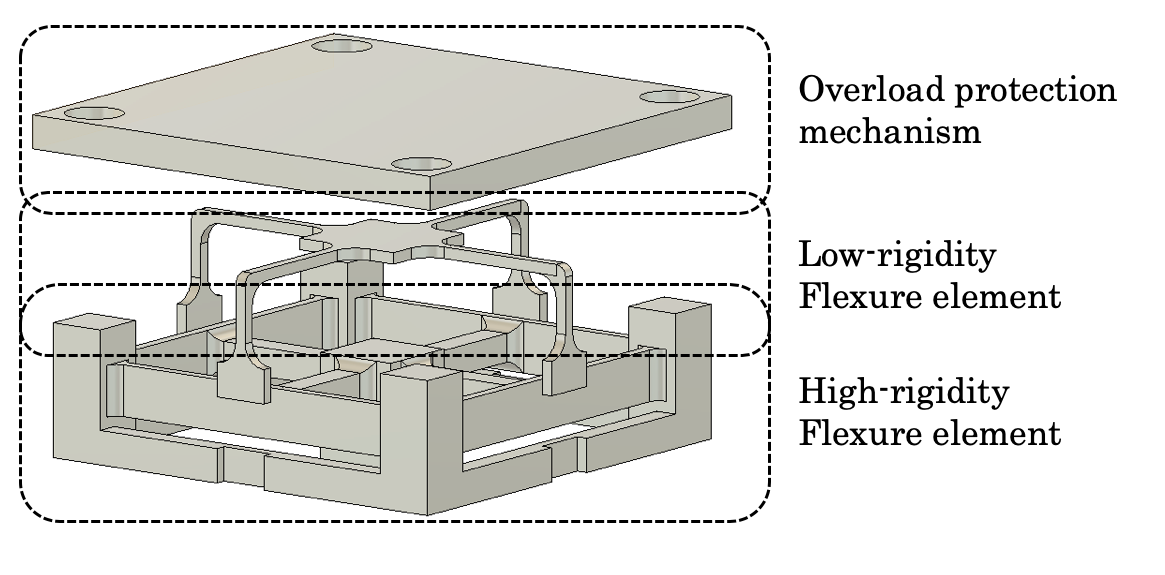
\includegraphics[width=6.0cm]{pic/sensor.png}
    \caption{全体の構造}\label{fig:sensor}
  \end{center}
 \end{figure}
 \begin{figure}[b]
  \centering
  \subfloat[低剛性起歪体]{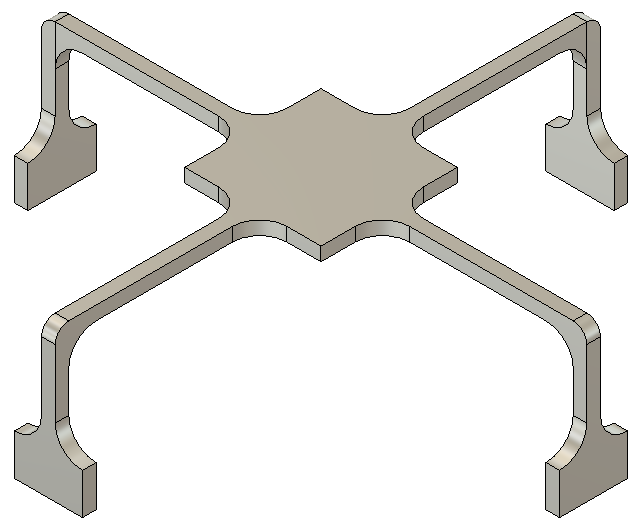
\includegraphics[width=3.5cm]{pic/LowCAD.png}}
  \subfloat[高剛性起歪体]{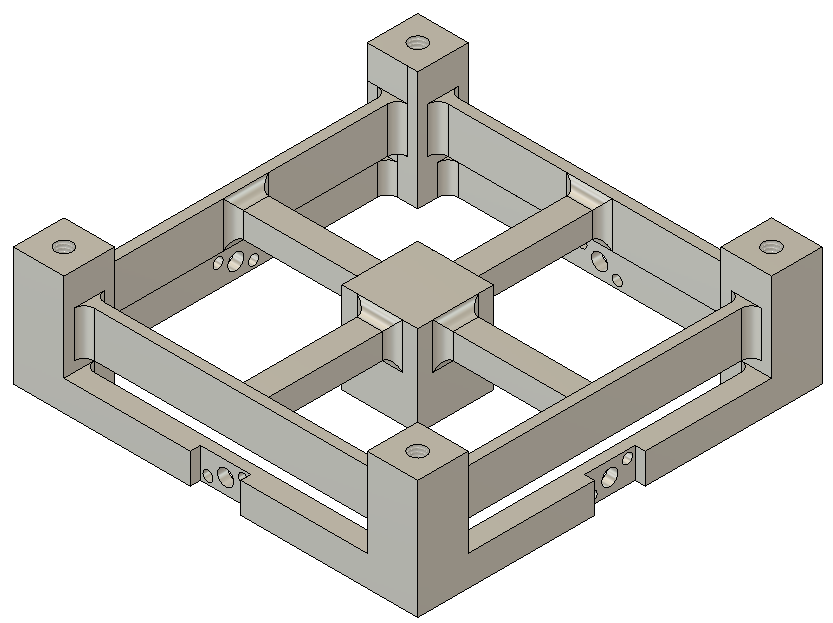
\includegraphics[width=3.5cm]{pic/HighCAD.png}}\\
  \caption[]{各起歪体の構造}\label{fig:kiwaitai}
\end{figure}
%\clearpage

\subsection{梁の設計}
力覚センサの中でも梁の構造はセンサ性能に大きく影響する重要な要素であり, 
その構造は任意の定格荷重, 荷重印加時のひずみ, 安全率といったパラメータを参考に決定される.
よって有限要素法シミュレーションにより荷重印加時の起歪体の挙動を調べた.

各起歪体に力と力のモーメント, 併せて6成分の定格荷重を印加した. 
この時の安全率をTable~\ref{tb:anzen}に示す. 
またFig.~\ref{fig:sim}に$-F_z$方向に力を加えた時の各起歪体の挙動を示す.
本力覚センサで設定した定格荷重はTable~\ref{tb:kajuu}に示す. 
\begin{table}[h]
  \caption{定格荷重($F$[N], $M$[Nm])}\label{tb:kajuu}
  \begin{center}
   \begin{tabular}{ c c c c c c c }
    \hline
     & $F_x$ & $F_y$ & $F_z$ & $M_x$ & $M_y$ & $M_z$  \\
    \hline
    Low-rigidity & 50 & 50 & 50 & 0.6 & 0.6 & 0.6  \\
    \hline
    High-rigidity & 500 & 500 & 500 & 10 & 10 & 12  \\
    \hline   
   \end{tabular}
  \end{center}
 \end{table}
\begin{table}[h]
  \caption{安全率\label{tb:anzen}}
  \begin{center}
   \begin{tabular}{ c c c c c c c }
    \hline
     & $F_x$ & $F_y$ & $F_z$ & $M_x$ & $M_y$ & $M_z$  \\
    \hline
    Low-rigidity & 2.04 & 2.04 & 1.83 & 1.78 & 1.78 & 3.13  \\
    \hline
    High-rigidity & 1.37 & 1.37 & 1.39 & 1.23 & 1.23 & 1.78  \\
    \hline   
   \end{tabular}
  \end{center}
 \end{table}
\subsection*{低剛性起歪体}
梁は低荷重に対して高感度である必要がある. よって, より細く長い梁が望ましい. 
しかし定格荷重を印加した時に塑性変形してしまう細さではいけない. 本力覚センサの低剛性起歪体の
梁の太さは2mm角に設計した. Fig.~\ref{fig:sim}~(a)より印加された荷重に対し
良好なひずみが得られたことがわかる. さらに, 6成分の定格荷重に対して
安全率が1以上を確保できている.
よって設計の妥当性が示された. 

\subsection*{高剛性起歪体}
高剛性起歪体の構造はクロスビーム型を参考としており,
外側剛体, 中央剛体, 弾性梁, 弾性薄板から構成される. 
弾性梁は5mm角で22.5mmの長さ, 弾性薄板は2mm厚, 9mm幅で56mmの長さである. 
Fig.~\ref{fig:sim}~(b)より印加された荷重に対し良好なひずみが得られたことがわかる. 
さらに, 6成分の定格荷重に対して安全率が1以上を確保できている. 
よって設計の妥当性が示された. 

設計した各起歪体の寸法をTable~\ref{tb:size} に示す. 
\begin{table}[h]
  \caption{起歪体の寸法[mm]}\label{tb:size}
  \begin{center}
   \begin{tabular}{ c c c c c }
    \hline
     & & Length & width & Height  \\
    \hline
    Low-rigidity & Body & 80 & 80 & 22  \\
    \cline{2-5}
     & Elastic bearn & 28 & 2 & 2  \\
    \hline
    High-rigidity & Body & 80 & 80 & 23.5  \\
    \cline{2-5}
     & Elastic bearn & 22.5 & 5 & 5  \\
    \cline{2-5}
     & Thin plate & 56 & 2 & 9 \\
    \hline
   \end{tabular}
  \end{center}
 \end{table}

\subsection{過負荷防止機構の構造}
過負荷防止機構の構造をFig.~\ref{fig:kahuka}に示す. 
過負荷防止機構はストッパピン, ストッパ板, 外側剛体(高剛性起歪体)から構成されている. 
6軸方向の各荷重に対し, 過負荷防止機構は以下のように動作する. 過負荷防止機構の作動荷重は
ストッパピン, ストッパ板, 外側剛体それぞれとのクリアランスによって決定される. 
本力覚センサのクリアランスの寸法をTable~\ref{tb:clea}に示す. 
\\
\begin{itemize}
  \item $\pm F_x$および$\pm F_y$:ストッパピンとストッパ板が接触. 
  \item $+F_z$:ストッパピンとストッパ板が接触. 
  \item $-F_z$:ストッパ板と外側剛体が接触. 
  \item $\pm M_x$および$\pm M_y$:ストッパ板がストッパピン, 外側剛体と接触
  \item $\pm M_z$:ストッパピンとストッパ板が接触. 
\end{itemize}
\begin{table}[h]
  \caption{過負荷防止機構のクリアランス[mm]}\label{tb:clea}
  \begin{center}
   \begin{tabular}{ c c }
    \hline
    Vertical clearance & Horizontal clearance  \\
    \hline
    0.3 & 0.3  \\
    \hline
   \end{tabular}
  \end{center}
 \end{table}

\subsection{ひずみゲージ貼付位置}\label{sec:hizumiharituke}
Fig.~\ref{fig:gage}に低剛性, 高剛性起歪体それぞれのひずみゲージの貼付位置を示す. 

ここで, 各起歪体にはそれぞれ$R_1~R_{16}$とラベリングされたひずみゲージが貼付されており, ()内に記されたひずみゲージは対となる
ひずみゲージの裏面に貼付されている. ひずみゲージは全て, 中央剛体から3mm離れた位置に配置されている.
ひずみゲージ$R_i$に生じるひずみ${\varepsilon} _i$とひずみ出力$S$は次のような関係で示せる. 
\begin{eqnarray}
  \left\{
    \begin{array}{l}
      S_{F_{x}} = \varepsilon _1 - \varepsilon _2 + \varepsilon _3 -\varepsilon _4 \\
      S_{F_{y}} = \varepsilon _5 - \varepsilon _6 + \varepsilon _7 -\varepsilon _8 \\
      S_{F_{z}} = \varepsilon _9 - \varepsilon _{10} + \varepsilon _{11} -\varepsilon _{12} \\
      S_{M_{x}} = \varepsilon _{13} - \varepsilon _{14} + \varepsilon _{16} -\varepsilon _{15} \\
      S_{M_{x}} = \varepsilon _{11} - \varepsilon _{12} + \varepsilon _{10} -\varepsilon _9 \\
      S_{M_{x}} = \varepsilon _5 - \varepsilon _6 + \varepsilon _8 -\varepsilon _7 \\
    \end{array}
  \right.\\ \nonumber
\end{eqnarray}
\begin{figure}[b]
  \centering
  \subfloat[低剛性起歪体]{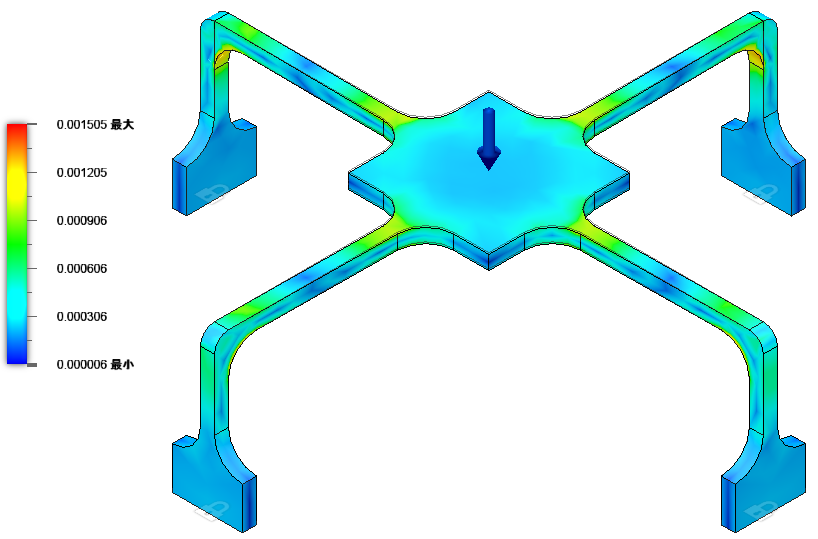
\includegraphics[width=6cm]{pic/Low_sim.png}}\\
  \subfloat[高剛性起歪体]{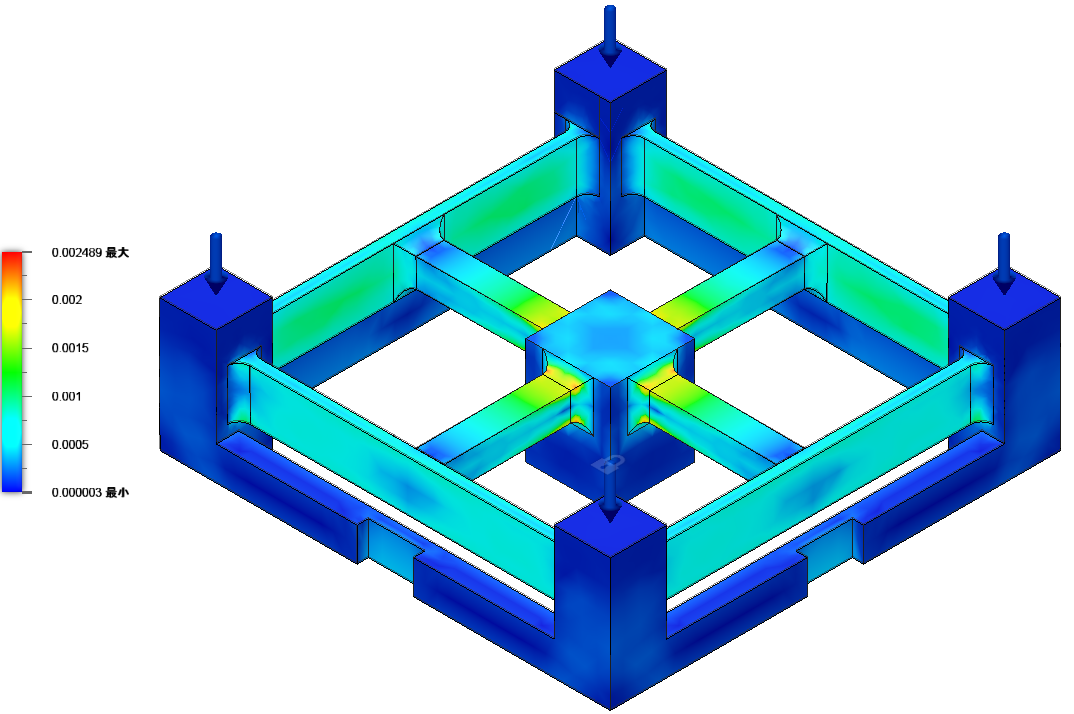
\includegraphics[width=6cm]{pic/High_sim.png}}\\
  \caption[]{有限要素法シミュレーションによる結果}\label{fig:sim}
\end{figure}
\begin{figure}[b]
  \centering
  \subfloat[側面]{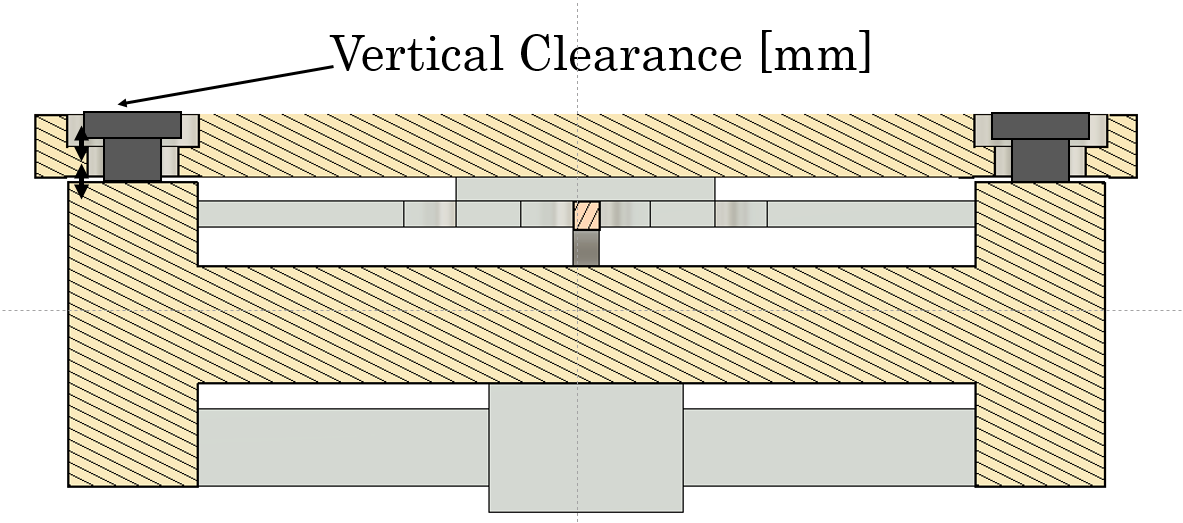
\includegraphics[width=4.25cm]{pic/Vertical.png}}
  \subfloat[上面]{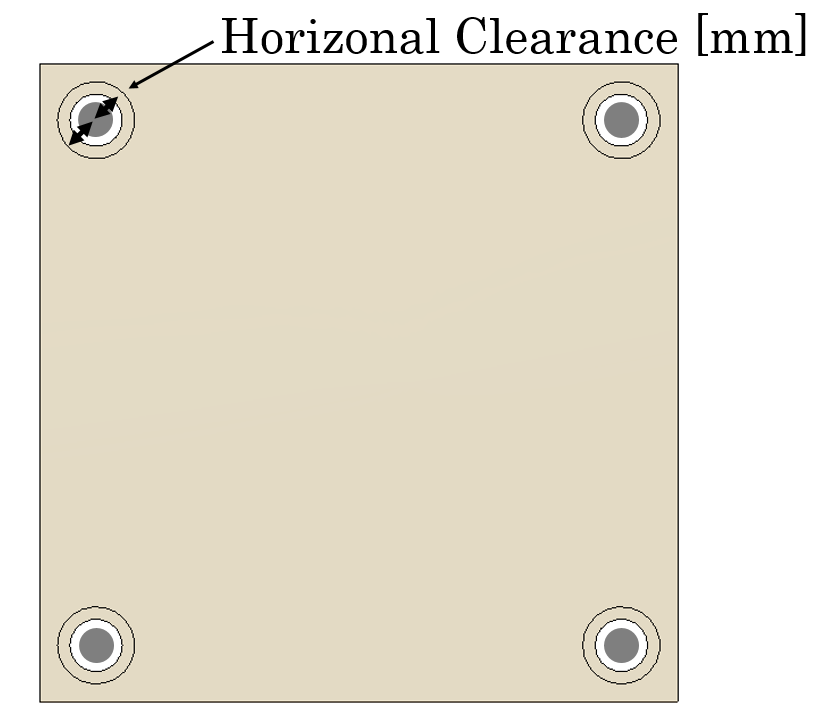
\includegraphics[width=4.2cm]{pic/Horizontal.png}}\\
  \caption[]{過負荷防止機構}\label{fig:kahuka}
\end{figure}
\begin{figure}[b]
  \centering
  \subfloat[低剛性起歪体]{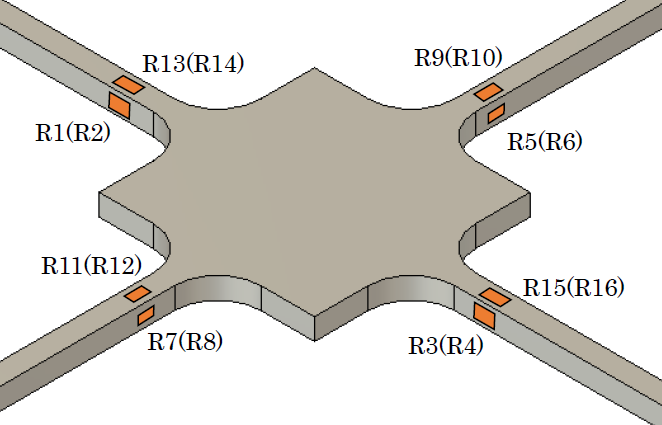
\includegraphics[width=4.3cm]{pic/LowGage.png}}
  \subfloat[高剛性起歪体]{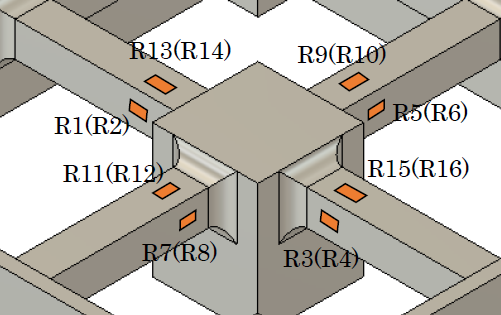
\includegraphics[width=4.3cm]{pic/HighGage.png}}\\
  \caption[]{ひずみゲージの貼付位置}\label{fig:gage}
\end{figure}
\subsection{センサ出力}
本力覚センサは印加荷重によって負荷が伝達される起歪体が異なる.
よって低剛性起歪体と高剛性起歪体それぞれから出力信号が取得される.
2つの出力信号には非線形性, 他軸干渉, ヒステリシスといった誤差が含まれており, 
単に起歪体からの出力信号を切り替えるだけではセンサ出力に飛躍が生じる. これによりセンサを導入した
ロボットの制御性能の劣化が生じる危険がある. そこで次式を用い, 
2つの起歪体から得られる出力信号を切り替える. 
\begin{eqnarray}
  \bm{L}_{out} = \alpha \bm{C}^{-1}_L \bm{S}_{L}+\left( 1-\alpha \right)\bm{C}^{-1}_H \bm{S}_{H}
  \label{eq:kirikae}
\end{eqnarray}
ここで$\bm{C}^{-1}$と$\bm{S}$は荷重-ひずみ変換行列とひずみ出力であり,下添え字Lは低剛性, Hは高剛性を意味する. また, $\alpha$は出力信号の仕様比率を表す. 
$\alpha$は次の式で表される. 
\begin{eqnarray}
  \alpha = \left\{
    \begin{array}{ll}
      0 & (L > L^{st}_{th}) \\
      \frac{ L^{fin}_{th} - L }{ L^{fin}_{th} - L^{st}_{th} } & (L^{st}_{th} < L < L^{fin}_{th})\\
      1 & (L < L^{fin}_{th})
      \label{eq:a}
    \end{array}
  \right.
\end{eqnarray}
ここで, $L^{st}_{th}$は切り替え開始の閾値, $L^{fin}_{th}$は切り替え終了の閾値となっている. 
また, 式\eqref{eq:kirikae}, 式\eqref{eq:a}を用いる事で,
\begin{enumerate}
  \item 印加荷重が$L^{st}_{th}$以下の場合:低剛性起歪体の出力のみ使用
  \item 印加荷重が$L^{st}_{th}$以上, $L^{fin}_{th}$以下の場合:飛躍した出力を抑制するため2つの出力を併用
  \item 印加荷重が$L^{fin}_{th}$以上の場合:高剛性起歪体の出力のみを使用
\end{enumerate}
といったようにセンサ出力が決定できる. 